\documentclass[letterpaper,oneside,12pt]{book}
\usepackage{graphicx}
\usepackage[american]{babel}

\selectlanguage{american}

% page layout
  \setlength{\hoffset}{-2.7cm} 
  \setlength{\voffset}{-.7in}
  \setlength{\textwidth}{15cm}
  \setlength{\oddsidemargin}{3.5cm}
  \setlength{\evensidemargin}{0.2cm}
  %\setlength{\topmargin}{2.5cm}
  \setlength{\headsep}{5ex}
\setlength{\textheight}{22cm}
  \renewcommand{\baselinestretch}{1.05}
\raggedbottom
  \newlength{\pictheight}
  \setlength{\pictheight}{\textheight}
  \addtolength{\pictheight}{-2cm}

% document
\begin{document}

\frontmatter
\begin{titlepage}
\hspace{-7mm}
\begin{minipage}{\textwidth}
\begin{center}
\vspace{.5cm}
{\huge \bf Software Design Document\\[1.5ex]}
{\large \bf for a specific implementation of `BCI2000'}
\\[1.5cm]
{\Large Gerwin Schalk\\}
{\Large Thilo Hinterberger\\}
{\Large Dennis J. McFarland\\[1.5cm]}
%
\begin{minipage}{13cm}
  \begin{minipage}[c]{13cm}
    \begin{center}
      {\Large \bf New York State Department of Health\\[2ex]}
      {\large \bf Wadsworth Center\\[0.5ex]
       Laboratory of Nervous Systems Disorders\\[4ex]}
      {\Large \bf Eberhard--Karls--Universit\"at T\"ubingen\\[2ex]}
      {\large \bf Medizinische Fakult\"at\\[0.5ex]
       Institut f\"ur Medizinische Psychologie\\[0.5ex]}
    \end{center}
  \end{minipage}
  \\[1.0cm]
  \begin{minipage}[c]{6cm}
    \centerline{
\includegraphics{figures/DOHlogo}}
  \end{minipage}
  \hspace{1.5cm}
  \begin{minipage}[c]{3cm}
    \centerline{
\includegraphics{figures/EKUlogo}}
  \end{minipage}
\end{minipage}
%
\\[0.5cm]
\textbf{Sponsors} \\
\textit{Jonathan R. Wolpaw and Niels Birbaumer}
\\[1.0cm]
{Albany, NY} \\[1ex]
{February 2000--May 2001}
\\[1ex]Updated May 2003, J\"urgen Mellinger
\end{center}
\end{minipage}
\end{titlepage}


\tableofcontents

\mainmatter

\chapter{Introduction}

\section{Involved Groups}

This document describes a joint project between the Lab of Nervous Systems 
Disorders, which is part of the Wadsworth Center in the New York State 
Department of Health, and the Institut f\"ur Medizinische Psychologie at the 
Eberhard--Karls--Universit\"at T\"ubingen.

\section{Project Heads}

The heads of this project are Jonathan R. Wolpaw, MD, and Prof. Dr. phil. Niels 
Birbaumer.

\section{Project Manager}

Gerwin Schalk, MS, has been assigned to be the project coordinator for this 
project. His responsibilities are to synchronize the combined effort of both 
groups, to report to the project heads, and to participate in the engineering.

\section{Project Team}

The project team consists of:
%\vspace{2ex}
\begin{itemize}
 \item{Thilo Hinterberger, Dr.}
 \item{Dennis McFarland, PhD}
 \item{Gerwin Schalk, MS}
\end{itemize}


\section{Acknowledgement}

We want to thank Dr. Jouri Perelmouter for his valuable input during the 
project design phase.


\chapter{Context and Objectives}

\section{Context}

In recent years, BCI development matured from bold experiments, performed by 
very few groups, to serious research undertaken by many facilities around the 
world. While all try to use cortical signals to provide a new communication 
channel for a severely handicapped population, they use many different 
physiological phenomena and methodologies to utilize these.

At the moment, the maximum rate of communication is 10-20 bits per minute. 
Because there is no commonly used shared platform, little is known about the 
efficacy of combining these phenomena in order to increase the information 
transfer rate.

In addition, very few groups currently apply BCI technology to the intended 
target population. In addition to technical difficulties, only a few facilities 
possess the necessary resources, e.g., the wide range of occupations, from 
engineers to psychologists to patient care personnel. An actual application that 
provided some - even if limited - useful function for patients, who could not be 
helped by conventional methods, could generate more interest towards this 
technology, and thereby foster further development.

\section{Objectives}

\subsection{Introduction}

The planned project addresses the aforementioned issues. The main goals are to 
produce a system in a reasonable time (i.e., by the end of 2000) that can be 
controlled by both mu/beta and/or slow potentials. The technical realization 
should make it easy for other groups to use/extend it to incorporate other 
physiological signals (e.g., P300). Furthermore, parts of the system (e.g., the 
operator) should be able to reside at a different physical location from the 
user.

\subsection{Details}

The following list shows the objectives in more detail. Although a major focus 
will be on a modular and flexible system, the technical realization has to be 
feasible. (This is not a programming contest for computer science gurus !!) 

\begin{itemize}
 \item{Different brain signal components, derived from (with a clear focus on mu/beta and slow potentials):}
    \begin{enumerate}
      \item{mu/beta}
      \item{slow cortical potentials}
      \item{P300}
      \item{SSVERs}
      \item{single units}
    \end{enumerate}
 \item{Open standard:}
    \begin{enumerate}
      \item{clear and documented interfaces between modules}
      \item{flexible file formats}
      \item{the programming environment should facilitate add-ons and changes by other groups}
    \end{enumerate}
 \item{Network capabilities, allowing the operator to be at a different physical location from the user}
\end{itemize}


\chapter{Project Plan}

\section{Work Breakdown Structure}

\begin{figure}[ht]
 \centerline{\scalebox{0.45}{\includegraphics{figures/WBS}}}
 \caption{The work breakdown structure for BCI2000}
\end{figure}


%\section{Responsibility Chart}


%\section{Gantt Chart}

%\begin{figure}[ht]
% \centerline{\scalebox{0.6}{\includegraphics{figures/GANTT.eps}}}
% \caption{The GANTT chart for BCI2000}
%\end{figure}


\section{Milestones}

\begin{tabular}{|c|l|l|}
 \hline
 \textbf{Milestone} & \textbf{Description} & \textbf{Reached}\\
 \hline
 1 & Empty shells and feasibility study & April 10, 2000\\
 \hline
 2 & Class model for signal processing & May 1, 2000\\
 \hline
 3 & Data acquisition & September 14, 2000\\
 \hline
 4 & Signal Processing & December 1, 2000\\
 \hline
 5 & User Application & March 1, 2001\\
 \hline
 6 & Bugfixes, analysis tools; transition to V1.0 & not yet\\
 \hline
\end{tabular}


\chapter{System Design} 

\section{Introduction}

This chapter describes the BCI2000 standard from the technical perspective. The 
level of detail should allow creation of a BCI2000-compliant module or an entire 
BCI2000 system implementation in any programming language and on any operating 
system platform.

The description is amplified to facilitate understanding by readers others than 
programmers.


\section{Overview}

\begin{figure}[ht]
 \centerline{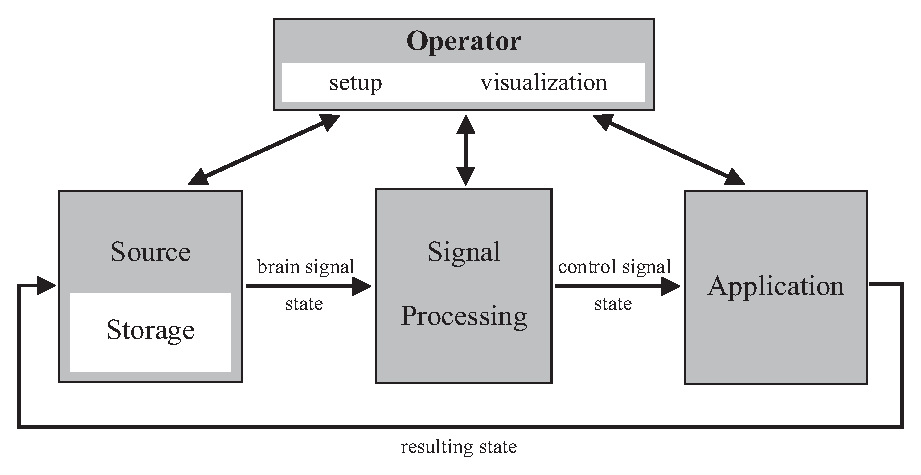
\includegraphics{figures/modules}}
 \caption{The functional modules and their interfaces}
 \label{fig:modules}
\end{figure}

Figure \ref{fig:modules} shows modules called \textit{Source}, \textit{Signal 
Processing}, \textit{Application}, and \textit{Operator}. We will refer to the 
three modules Source, Signal Processing and Application together as \textit{core 
modules}.


%\section{Functional Modules}


\section{Core--Operator Communication}

\subsection{Introduction}

The same communication protocol is used between each of the three core modules 
and the operator module. It is an asynchronous state-less application-level 
protocol. Although it can be implemented on top of any transport protocol, it 
assumes the reliability of TCP (i.e., the protocol does not support 
acknowledgements or packet sorting or any other means of error correction).

Any message sent to or from any module is wrapped into packets as described in 
section \ref{protocol_definition}. This simple protocol allows for the delivery 
of data (e.g., parameters, visualization data, etc.), even if its content and 
nature are not known \textit{a priori}.


\subsection{Protocol Definition}
\label{protocol_definition}

Communication consists of messages that are sent and received asynchronously 
between any core module and the operator module. Each message starts with a one-
byte content descriptor and one-byte descriptor supplement, followed by a 16-bit 
unsigned integer (little endian) that describes the length of the content.

\begin{figure}[ht]
 \centerline{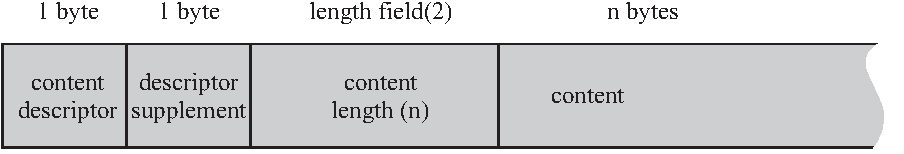
\includegraphics{figures/operator_prot}}
 \caption{Layout of one message in the protocol}
\end{figure}

\begin{table}[ht]
 \centering
 \begin{tabular}{|l|l|}
  \hline
  \textbf{descriptor} & \textbf{description} \\
  \hline
  1 & status information string \\
  \hline
  2 & system parameter \\
  \hline
  3 & system state \\
  \hline
  4 & visualization data \\
  \hline
  5 & state vector \\
  \hline
  6 & system command \\
  \hline
 \end{tabular}
 \caption{The currently defined content descriptors}
\end{table}   


\subsection{Descriptor=1: Status Information Format}
\label{statusinfo_format}

This section describes the format of the message when the core message is 
a status information string (i.e., the message's descriptor is 1). In this 
case, the aforementioned content data is a line of ASCII characters 
in the following format:
\\[2ex]
xxx: status--line--text 
\\[2ex]
xxx is a three digit number that describes the content of the status information string. 
The first digit is '1' for status information, '2' for successful operation, '3' 
for recoverable errors and '4' for fatal errors. The two remaining digits define 
the exact nature of the message, followed by a plain description.

This procedure is used to communicate errors and to convey status information (e.g.,
the operator module may display the remaining disc space on the Source module's
machine.)

\subsection{Descriptor=2: Parameter Format}
\label{parameter_format}

This section describes the format of the message when the core message is of 
type system parameter (i.e., the message's descriptor is 2). In this case, the 
aforementioned content data is a line of ASCII characters (parameters delimited 
by spaces) in the following format (Table \ref{tab:parametervariables} summarizes
the individual components in the parameter string):
\\[2ex]
Section DataType Name= Value DefaultValue LowRange HighRange // Comment CRLF \\[2ex]
If DataType is \textit{list, intlist} or \textit{floatlist}, the format is
as follows: 
\\[2ex]
Section DataType Name= (NumValues$\mid${Labels}) Value(s) DefaultValue LowRange HighRange // Comment CRLF \\[2ex]
where Labels is a list of textual labels that optionally substitutes the number denoted by NumValues. A list of labels is enclosed in a matching pair of any of \verb|{}, [], (), <>|, as in 
\verb|[low medium high]|.
\\[2ex]
If DataType is \textit{matrix}, the format is as follows:
\\[2ex]
Section DataType Name= (NumValuesDim1$\mid$LabelsDim1) (NumValuesDim2$\mid$LabelsDim2) Value(s) DefaultValue LowRange HighRange // Comment CRLF \\[2ex]
where again each NumValues entry may be substituted by a list of textual labels.

This format not only applies to the interaction between core and operator, but
also reflects the data format of the system's parameter files (i.e., files with
extension .prm). The core modules and the operator module use this format to
communicate in the system initialization phase (as described in section \ref{system_init}).

\begin{table}[ht]
 \centering
 \begin{tabular}{|l|l|}
  \hline
  \textbf{Name} \\
  \hline
  Section \\
  \hline
  Type \\
  \hline
  Name \\
  \hline
  ${\left[
    \mbox{(NumValuesDim1$\mid$\{ LabelDim1.1 LabelDim1.2 ... \})}
    \atop
    \mbox{[(NumValuesDim2$\mid$\{ LabelDim2.1 LabelDim2.2 ... \})]}
    \right]}$ \\
  \hline
  Value(s) \\
  \hline
  DefaultValue \\
  \hline
  LowRange \\
  \hline
  HighRange \\
  \hline
  Comment \\
  \hline
 \end{tabular}
 \caption{Definition of variables in the parameter string}
 \label{tab:parametervariables}
\end{table}   

If \textit{NumValues} is provided (i.e., data type \textit{list, intlist} or 
\textit{floatlist}), it indicates how many values are following it. The separate 
values are then delimited by white spaces. In case of data type \textit{matrix}, 
the transmitted values represent the matrix as follows: the first NumValuesDim2 
values are value(0, t), followed by NumValuesDim2 values value(1, t), etc.;
in case that labels are specified in place of value counts, the analogy holds
with the value counts given by the number of labels for the dimension in
question.\\

Each core module knows the data types of the parameters it is requesting and 
thus does not need a parameter data type definition. However, the operator 
module uses the data type definitions as listed in the table below to create 
their graphical representation. Section \ref{system_params} describes a list of 
pre-defined system parameters.


\subsection{Descriptor=3: State Format}
\label{state_format}

This section describes the format of the message when the core message is of 
type system state (i.e., the message's descriptor is 3). In this case, the 
aforementioned content data is a line of ASCII characters (parameters
delimited by spaces) in the following format:
\\[2ex]
Name Length Value ByteLocation BitLocation CRLF
\\[2ex]
with ByteLocation between 0..29 and BitLocation ranging from 0..7. The core 
modules and the operator module use this format to communicate in the system 
initialization phase (as described in section \ref{system_init}), as well as 
during system performance (section \ref{system_performance}) and for system 
termination (section \ref{system_termination}). Table \ref{state_table} 
defines the maximum length for each parameter.

\begin{table}[ht]
 \centering
 \begin{tabular}{|l|l|}
  \hline
  \textbf{Name} & \textbf{Max. Length} \\
  \hline
  Name & 30 \\
  \hline
  Length & 2 \\
  \hline
  Value & 5 \\
  \hline
  ByteLocation & 1 \\
  \hline
  BitLocation & 1 \\
  \hline
 \end{tabular}
 \caption{Definition for variables in the state string}
 \label{state_table}
\end{table}   

\subsection{Descriptor=4: Visualization Data Format}
\label{visualizationdata_format}

This section describes the format of the message when the core message is of 
type visualization data (i.e., the message's descriptor is 4). In this case (see 
figure \ref{visualizationprotocol}), the content descriptor describes the 
requested visualization type. The only currently defined types are 1 (a graph of 
\textit{n} channels and \textit{m} samples) and 2 (a text memo). Other (not yet 
defined) types could be Horizontal Ball, Vertical Ball, Speller Status, etc. A 
visualization type of 255 defines visualization configuration.

\begin{figure}[ht]
 \centerline{\scalebox{0.75}{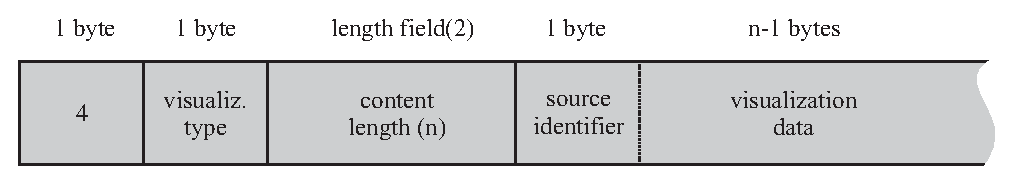
\includegraphics{figures/operator_prot_visualization}}}
 \caption{One message in the protocol, if it is of type "visualization data"}
 \label{visualizationprotocol}
\end{figure}

\begin{figure}[ht]
 \centerline{\scalebox{0.75}{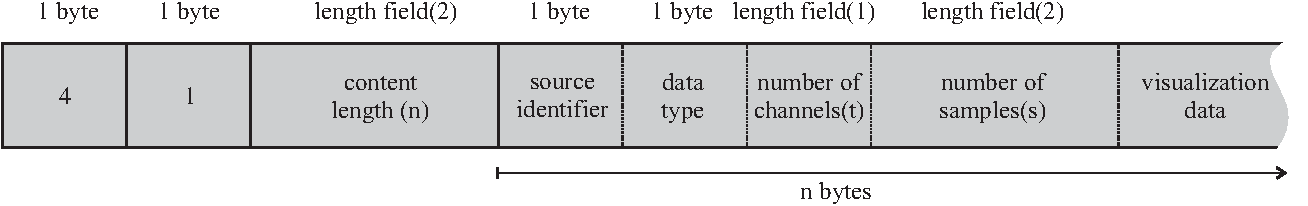
\includegraphics{figures/operator_prot_visualization_type1}}}
 \caption{One message, if visualization type is 1 (i.e., a graph)}
 \label{visualizationprotocol_type1}
\end{figure}

Figure \ref{visualizationprotocol_type1} illustrates the protocol when the 
visualization type is 1. The source identifier defines a unique number 
identifying the process/filter that generated the data. The data type can be 
either 0 (for integers in little endian format) or 1 (for floating-point 
values); the number of channels and samples are self explanatory. Floating point 
values are transmitted as three bytes each. The first two bytes (i.e., A) define 
the mantissa (signed two-byte integers in little endian format) and the third 
byte (i.e., B) defines the exponent (signed one-byte integer). The actual floating 
point value is then calculated as follows: $value=A*10^{B}$. Figure 
\ref{visualization_type1} illustrates how the data is transferred.

\begin{figure}[ht]
 \centerline{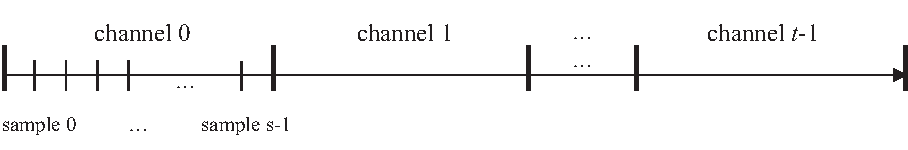
\includegraphics{figures/visualization_type1}}
 \caption{Graphical representation of the transmitted visualization data format}
 \label{visualization_type1}
\end{figure}

\begin{figure}[ht]
 \centerline{\scalebox{0.75}{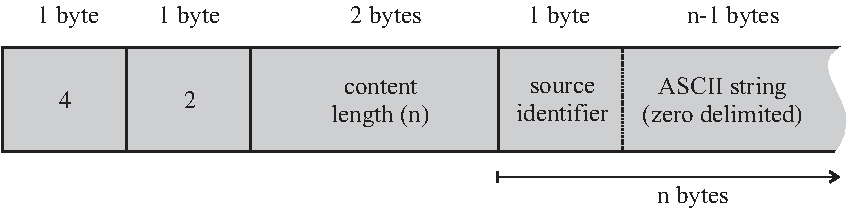
\includegraphics{figures/operator_prot_visualization_type2}}}
 \caption{One message, if visualization type is 2 (i.e., a text memo)}
 \label{visualizationprotocol_type2}
\end{figure}

Figure \ref{visualizationprotocol_type2} illustrates the protocol when the 
visualization type is 2. The source identifier defines a unique number 
identifying the process/filter that generated the data. The following ASCII
text is zero delimited.

\begin{figure}[ht]
 \centerline{\scalebox{0.75}{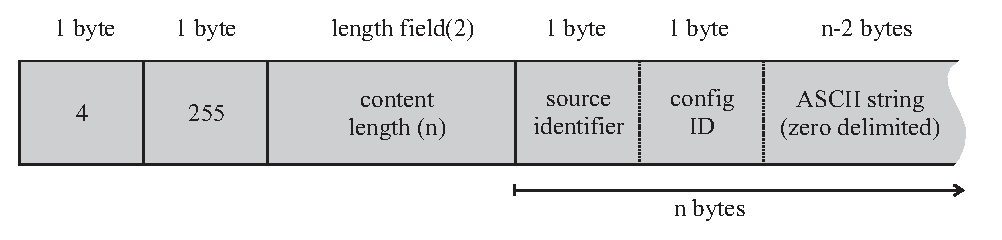
\includegraphics{figures/operator_prot_visualization_type255}}}
 \caption{One message, if visualization type is 255 (i.e., visualization configuration)}
 \label{visualizationprotocol_type255}
\end{figure}

Figure \ref{visualizationprotocol_type255} illustrates the protocol when the 
visualization type is 255. The source identifier defines a unique number 
identifying the process/filter that generated the data. The different 
configuration IDs are described in Table \ref{tab:viscfg_table}.

\begin{table}[ht]
 \centering
 \begin{tabular}{|l|l|}
  \hline
  \textbf{Cfg ID} & \textbf{Description} \\
  \hline
  1 & Window Title \\
  \hline
  2 & Minimum Value \\
  \hline
  3 & Maximum Value \\
  \hline
  4 & Number of Samples \\
  \hline
  5 & X Axis Lable \\
  \hline
  6 & Y Axis Lable \\
  \hline
 \end{tabular}
 \caption{The various IDs for visualization configuration}
 \label{tab:viscfg_table}
\end{table} 

The ASCII string then contains the configuration option, as defined by the 
configuration ID. For example, it might contain "128", if the configuration ID 
is 4. This will configure the graph to contain exactly 128 samples. When the 
configuration ID is 5 or 6 (axis labels), the ASCII string consists of a sample 
number (three digits), a space, and the axis label. Thus, one message configures 
exactly one axis label. As an example and for an X-axis label, the string "003 
4.75 Hz" would result in a graph, in which the third sample is labeled "4.75 
Hz."


\subsection{Descriptor=5: State Vector}
\label{statevector}

This section describes the format of the message when the core message is of 
type state vector (i.e., the message's descriptor is 5). 

The state vector is defined by a series of \textit{StateVectorLength} subsequent 
bytes. The structure of these bytes is defined in \ref{statevector_format}.


\subsection{Descriptor=6: System Command}
\label{sec:syscmd}

This section describes the format of the message when the core message is of 
type system command (i.e., the message's descriptor is 6). 

The system command consists of an ASCII string that may end with a zero byte 
(i.e., ASCII code 0).

The nature of these system commands is defined by the specific implementation of 
the modules.


\section{Inter--Core Communication}

\subsection{Introduction}

Unlike the bidirectional communication between core modules and the operator 
module, communication within the core modules is unidirectional. The initial 
setup determines the exact nature of this communication and data is transmitted 
with the same protocol as described in Section \ref{protocol_definition}. The 
following sections describe the transferred brain signal, state vector, and 
control signal. The state vector must always be transmitted before the brain 
signal or control signal. Whenever \textit{Running} switches from 0 to 1, the 
system is re-initialized and the nature of the subsequently transmitted signals 
could change. Transmitting the state vector before the signals (brain signal or 
control signals) allows modules to react to these changes.

\subsection{Brain Signal Format}
\label{sec:eegsigformat}

The brain signal is transmitted similarly to visualization data (i.e., as 
described in Section \ref{visualizationdata_format}). The visualization type is 
set to 1 (i.e., graph), source identifier is set to 0, data type is integer 
(i.e., 0) and channels and samples are self-explanatory.


\subsection{State Vector Format}
\label{statevector_format}

The state vector is transferred as type state vector (see Section 
\ref{statevector}). The content descriptor is 5 and the descriptor supplement is 
undefined. Its content consists of a series of \textit{StateVectorLength} bytes. 
The value of a given state within the state vector is determined by its byte/bit 
location and length definition. The bits in the state vector are always sorted 
in ascending order, e.g., for a state with a length of 7 bits, starting at byte 
location 2, bit location 3, bit zero is first (byte 2, bit 3), and the highest 
bit (bit 7) is last (byte 3, bit 1).


\subsection{Control Signal Format}

Control signals are transmitted similarly to the Brain Signal (see Section 
\ref{sec:eegsigformat}) with \textit{NumControlSignals} channels and 1 sample 
per channel.


\section{System--Wide Parameters}
\label{system_params}

\subsection{Introduction}

System--wide parameters are published and initialized during system--startup, as 
described in section \ref{system_init}. Each parameter is described by the 
section it belongs to, a data type descriptor, its name, value(s), default 
value, and a range of valid numbers. Parameter names are unique across the 
entire system.

\subsection{Reserved Data Types}

\vspace{.5cm}

\begin{flushleft}

\begin{centering}
 \begin{tabular}{|l|l|}
  \hline
  \textbf{Data Type} & \textbf{Description} \\
  \hline
  char & one character \\
  \hline
  string & a string of characters \\
  \hline
  int & a 16-bit signed integer \\
  \hline
  longint & a 32-bit signed integer \\
  \hline
  float & a single--precision floating point \\
  \hline
  bool & a boolean value (0..false, 1..true) \\
  \hline
  intlist & a list of 16-bit signed integer \\
  \hline
  floatlist & a list of single-precision floating points \\
  \hline
  matrix & a matrix of single-precision floating points \\
  \hline
 \end{tabular}
% \caption{Data type definition for variables in the parameter string}
\end{centering}   

\vspace{.5cm}

\newpage

\subsection{Reserved Sections and Parameter Names}

Several section descriptors are currently defined. They are:

\begin{flushleft}
% \centering
 \begin{tabular}{|l|}
  \hline
  \textbf{Section Name}\\
  \hline
  Source \\
  \hline
  Storage \\
  \hline
  Filtering \\
  \hline
  Classification \\
  \hline
  Statistics \\
  \hline
  Task \\
  \hline
  Sequencer \\
  \hline
  Visualization \\
  \hline
  System \\
  \hline
 \end{tabular}
% \caption{The currently defined section descriptors}
\end{flushleft}

\raggedright Listed below are all currently defined sections with their reserved parameter 
names.
\\[2ex]
\raggedright \large Section "Source" \normalsize
\\[2ex]
%\begin{displaymath}
 \begin{tabular}{|l|l|l|}
  \hline
  \textbf{Type} & \textbf{Parameter Name} & \textbf{Description}\\
  \hline
  int & SoftwareCh & number of digitized and stored channels \\
  \hline
  int & SampleBlockSize & number of transmitted samples \\
  \hline
  intlist & SourceChList & list of source channels \\
  \hline
  int & TransmitCh & number of transmitted channels \\
  \hline
  intlist & TransmitChList & list of channels to transmit \\
  \hline
  floatlist & SourceChOffset & offset in A/D units\\
  \hline
  floatlist & SourceChGain & factor to convert A/D units to $\mu$V \\
  \hline
  int & SamplingRate & data acquisition's sampling rate in Hz \\
  \hline
 \end{tabular}
 %\caption{Parameter names in section Source}
%\end{displaymath}

\vspace{.5cm}
\raggedright \large Section "Storage" \normalsize
\\[2ex]
%\begin{displaymath}
 \begin{tabular}{|l|l|l|}
  \hline
  \textbf{Type} & \textbf{Parameter Name} & \textbf{Description}\\
  \hline
  string & SubjectName & subject alias (max. 8 characters) \\
  \hline
  string & SubjectSession & session number (max. 3 characters) \\
  \hline
  string & SubjectRun & digit run number (max. 3 characters) \\
  \hline
  string & FileName & name (w/o ext) for data file (max. 32 char.)\\
  \hline
  int & StorageMethod & \\
  \hline
  int & StorageTime & \\
  \hline
 \end{tabular}
% \caption{Parameter names in section Storage}
%\end{displaymath}

\vspace{.5cm}
Parameter names in section Filtering and Classification are preceded by 
a two--character identifier that indicates the type of the parameter.

\vspace{.5cm}

\newpage

\large Section "Filtering" \normalsize \\[1ex]

%\begin{table}[!ht]
 \begin{tabular}{|l|l|l|}
  \hline
  \textbf{Type} & \textbf{Parameter Name} & \textbf{Description}\\
  \hline
  int & NumControlSignals & number of transmitted control signals \\
  \hline
  & SWxxx & slow--wave filtering \\
  \hline
  & FTxxx & Fourier transform \\
  \hline
  & SPxxx & other spectral analysis methods \\
  \hline
 \end{tabular}
% \caption{Parameter names in section Filtering}
%\end{table}   

\vspace{.5cm}
\large Section "Classification" \normalsize \\[1ex]

%\begin{table}[!ht]
 \begin{tabular}{|l|l|l|}
  \hline
  \textbf{Type} & \textbf{Parameter Name} & \textbf{Description}\\
  \hline
   & LDxxx & linear discriminant analysis \\
  \hline
   & NNxxx & neural network classifier \\
  \hline
 \end{tabular}
% \caption{Parameter names in section Classification}
%\end{table}   

\vspace{.5cm}
\large Section "Sequencer" \normalsize \\[1ex]

%\begin{table}[!ht]
 \begin{tabular}{|l|l|l|}
  \hline
  \textbf{Type} & \textbf{Parameter Name} & \textbf{Description}\\
  \hline
 \end{tabular}
% \caption{Parameter names in section Sequencer}
%\end{table}   

\vspace{.5cm}
\large Section "Visualization" \normalsize \\[1ex]

%\begin{table}[!ht]
 \begin{tabular}{|l|l|l|}
  \hline
  \textbf{Type} & \textbf{Parameter Name}\\
  \hline
  int & ViewSourceCh[SoftwareCh, ViewSourceBlockSize]\\  
  \hline
  int & ViewTransmitCh[TransmitCh, ViewTransmitBlockSize]\\
  \hline
  int & ViewControlCh [ControlCh, ViewControlBlockSize] \\
  \hline
  float & ViewFFTCh[FFTCh, ViewFFTBlockSize] \\
  \hline
  float	& ViewSWCh[SWCh, ViewSWBlockSize] \\
  \hline
 \end{tabular}
% \caption{Parameter names in section Visualization}
%\end{table}   

\vspace{.5cm}
\large Section "System" \normalsize \\[1ex]

%\begin{table}[!ht]
 \begin{tabular}{|l|l|l|}
  \hline
  \textbf{Type} & \textbf{Parameter Name} & \textbf{Description}\\
  \hline
  string & EEGsourceIP & the IP address the EEGsource core module listens on\\  
  \hline
  int & EEGsourcePort & the port the EEGsource core module listens on\\  
  \hline
  string & SignalProcessingIP & the IP address the SignalProcessing core module listens on\\  
  \hline
  int & SignalProcessingPort & the port the SignalProcessing core module listens on\\  
  \hline
  string & ApplicationIP & the IP address the Application core module listens on\\  
  \hline
  int & ApplicationPort & the port the Application core module listens on\\  
  \hline
  int & StateVectorLength & the length of the state vector in bytes\\  
  \hline
 \end{tabular}
% \caption{Parameter names in section System}
%\end{table}   

\end{flushleft}


\section{System-Wide States}
\label{states}

\subsection{Introduction}

While the purpose of system--wide parameters is to define the static 
configuration, the state information provides dynamic information about the 
current state of the system, e.g., whether the system is running or not.

States are published and initialized during system--startup, as described in 
section \ref{system_init}. A state is described by its name, its length (in 
bits) and its location (defined by start byte and bit in the state vector). 
The state vector is always transferred as a full number of bytes (specifically, 
\textit{StateVectorLength} bytes) (i.e., the end is padded with meaningless 
bits if necessary).

\subsection{The State Vector}

While the operator module constructs the state vector after receiving 
all requests for states from the core modules, some states do not need to be
to be requested -- they are created automatically. They are:
\\[2ex]
\begin{tabular}{|l|l|l|}
 \hline
 \textbf{Length} & \textbf{Name} & \textbf{Description}\\
 \hline
 16 & SourceTime & 16-bit unsigned integer (little endian); resolution 1 ms \\  
 \hline
 16 & StimulusTime & 16-bit unsigned integer (little endian); resolution 1 ms \\  
 \hline
 1 & Online & 1: A/D or random input, 0: input from file \\  
 \hline
 1 & Running & 1: system is running, 0: system is suspended\\  
 \hline
 1 & Recording & 1: system is recording, 0: not recording\\  
 \hline
 1 & RunActive & \\  
 \hline
 1 & BaselineInterval & Application is in baseline interval\\  
 \hline
 1 & FeedbackInterval & \\  
 \hline
 1 & InterTrialInterval & Application is between trials\\ 
 \hline
 1 & InterRunInterval & Application is between runs\\ 
 \hline
\end{tabular}


\section{System Initialization}
\label{system_init}

\subsection{Introduction}

This section describes the system initialization process. Since the system is a 
distributed system of encapsulated modules, this procedure ensures a proper and 
well defined information flow at start-up.

\subsection{Startup Sequence}

The operator module must be started first. Since in most cases the IP address of 
the operator module can be more easily statically defined, its IP address and 
port number(s) have to be provided to the core modules. It listens on ports 4000 
(for Source), 4001 (for Signal Processing), and 4002 (for Application) and 
waits for the respective core module to connect. Each can connect to its 
assigned port on the operator module in any order. Upon start--up, each core 
module opens a listening socket on any arbitrary port number.

\subsection{Publishing Phase}

Upon connection, each core module publishes its parameters to the operator 
module, as described in section \ref{parameter_format}. After publishing its 
parameters, each core module publishes its requested states, as described in 
chapter \ref{state_format}. At this time, the operator module ignores every 
field except \textit{Name} and \textit{Length}, which it needs to construct the 
state vector.

For this and all subsequent communication, the modules use the protocol 
described in chapter \ref{protocol_definition}. Each core module sends a state 
with the name \textit{EndOfState} as the last state. The operator module does 
not process this state. On receiving this state from all core modules, it ends 
this initial publishing phase.

\subsection{Information Phase}

The operator module processes the received parameters and states. It creates a 
list of all parameters and all states and creates the state vector (double 
parameters or states are ignored). At this point, the operator module may modify 
the value of the parameters and states (depending on the investigator's input or 
the parameter file). The operator module then uses the same channel on which it 
received data from the core modules to send back to all core modules a list of 
all system--wide parameters and system-wide states (in any order). Since the IP 
address and port number on which the core modules listen for data from other 
core modules are published in system parameters as described, each module now 
knows where to send its data. The connections from the core modules to the 
operator module remain open (all subsequent traffic will go through these 
connections.)

As in the publishing phase, the Information Phase ends when a state 
\textit{EndOfState} is sent.

In order to maintain integrity throughout operation, no parameters or states 
should be added to or removed from the system beyond this point.

\subsection{Preflight Phase}
\textit{Note: As of May 2003, the Preflight phase is not fully implemented,
so the information in this paragraph is not accurate for the actual module
code.--jm}\\[1ex]
Each core module declares whether it can process data with the received
parameters and states, or indicates errors by sending descriptions into
an error channel. If any errors are indicated during the preflight phase,
the operator module will not initiate the initialization phase but display
the errors, prompting the user to fix the problems detected.

\subsection{Initialization Phase}

Each core module uses the information in the received parameters to configure and 
initialize its operation. It also opens an active (i.e., client) connection 
to the other core module it must connect to, i.e., Source opens a 
connection to Signal Processing, Signal Processing to Application and 
Application to Source.

Each core module sends a status message (see \ref{statusinfo_format}) to the 
operator that indicates either successful or failed initialization. The 
Initialization Phase ends when all core modules indicate successful 
configuration.


\section{System is Running}
\label{system_performance}

At the end of the Initialization Phase, the system is fully configured. All 
parameters and states (and positions thereof in the state vector) are defined. 
During system operation, the Operator module must send states only to the Source 
module and Signal Processing and Application must disregard any state that the 
Operator does send to them. 

The system is started when the Operator module sets the state \textit{Running} 
to 1 and sends it to the Source module. 


\section{System is Suspended}
\label{sec:system_suspended}

The system is suspended when \textit{Running} is 0. Any module shall disregard a 
change in parameters if the system is not suspended. Data flows through the 
system and it is up to each module to decide how to process these data. The 
Application, for example, might give visual feedback that indicates that the 
system is suspended. As long as operation is suspended (i.e., \textit{Running} 
is 0), any module might update system parameters and send them back to the 
Operator.


\section{System Termination}
\label{system_termination}

If any module detects a dropped connection to the Operator, it must shut down 
all other socket connections and terminate.

\section{File Formats}

\subsection{Data File}

The data file consists of a header and the actual raw brain signals. The header 
consists of a definition of all system parameters and states. Thus, parameters 
must not change within one data file.

\subsubsection{Header}

The header of a data file consists of lines of ASCII characters. Its total 
length is determined by the parameter HeaderLen in the first line. The first 
line specifies general parameters, while the following define all states in the 
state vector, as well as all the current parameters. The number of bytes in the 
state vector is determined by the sum of the lengths (defined in bits) for all 
states, rounded up to the next byte (which equals the value of 
\textit{StateVectorLength} in both the first line and, since 
\textit{StateVectorLength} is also a system--wide parameter, in one of the lines 
in the [ParamDef] section). Thus, the data file can be read (although not fully 
interpreted) by reading the first line. The state definitions have the same 
format as described in \ref{state_format} (although their values in the header 
are irrelevant, since they are defined for each sample in the data file). The 
parameter definitions have the format described in section 
\ref{parameter_format}.

\begin{flushleft}
HeaderLen= length  SourceCh= m  StateVectorLength= k CRLF \\[1ex]
[StateVectorDef] CRLF \\[1ex]
Name1 Length1 Value1 ByteLocation1 BitLocation1 CRLF \\[1ex]
Name2 Length2 Value2 ByteLocation2 BitLocation2 CRLF \\[1ex]
Name3 Length3 Value3 ByteLocation3 BitLocation3 CRLF \\[1ex]
... \\[1ex]
[ParamDef] CRLF \\[1ex]
Section1 DataType1 Name1= Value1 DefaultValue1 LowRange1 HighRange1 // Comment CRLF \\[1ex]
Section2 DataType2 Name2= Value2 DefaultValue2 LowRange2 HighRange2 // Comment CRLF \\[1ex]
Section3 DataType3 Name3= Value3 DefaultValue3 LowRange3 HighRange3 // Comment CRLF \\[1ex]
... \\[1ex]
CRLF \\
\end{flushleft}
The binary data directly follows this last CRLF.

\subsubsection{Binary Data}
\label{binary_data}

\textit{SourceCh} data--channels, followed by \textit{StateVectorLength} bytes 
for the state vector. Data samples are stored as 16-bit signed integers (little 
endian). The number of samples in the file can be calculated as follows: 
$samples=\frac{filesize}{2*SourceCh+StateVectorLength}$.

\subsection{Parameter File}

A parameter file consists of lines of ASCII in the same format as the data file 
header and as described in section \ref{parameter_format}.

\newpage
\subsection{BCI2000 File Extensions}

The following table lists all extensions for BCI2000 data files:
\vspace{0.5cm}\\
\begin{centering}
 \centering
 \begin{tabular}{|l|l|}
  \hline
  \textbf{description} & \textbf{extension} \\
  \hline
  Data file & .dat \\
  \hline
  Parameter file & .prm \\
  \hline
  Application file & .app \\
  \hline
  Psychological state & .psy \\
  \hline
 \end{tabular}
 %\caption{Reserved extensions for BCI2000 data files}
\end{centering}   

\section{Glossary} 

\textbf{little endian} \\
In little endian, the binary representation of a 16-bit integer is: low-byte (bits 0-7)
first, followed by the high-byte (bits 8-15).
\\[2ex]
\textbf{CR} \\
stands for carriage return, or {ASCII} code 10.
\\[2ex]
\textbf{LF} \\
stands for line feed, or {ASCII} code 13.
\\[2ex]
\textbf{CRLF} \\
stands for carriage return and line feed, or (subsequent) {ASCII} codes 10 and 13.
\\[2ex]
\textbf{parameter} \\
A parameter is a static and global variable that describes some aspect of the 
system configuration. Parameters can only be created or changed during the 
system startup phase.
\\[2ex]
\textbf{state} \\
A state is a n--bit value that describes some aspect of the current system 
status. In communication, a state is represented as described in section
\ref{state_format}.
\\[2ex]
\textbf{state vector} \\
The state vector holds all values for all states that are packed together in one
array of bytes of length \textit{StateVectorLength}.


\backmatter
\end{document}

